\newpage
\section{Wasserkraft}


\subsection{Kontinuitätsgleichung des Durchflusses}
\begin{center}
    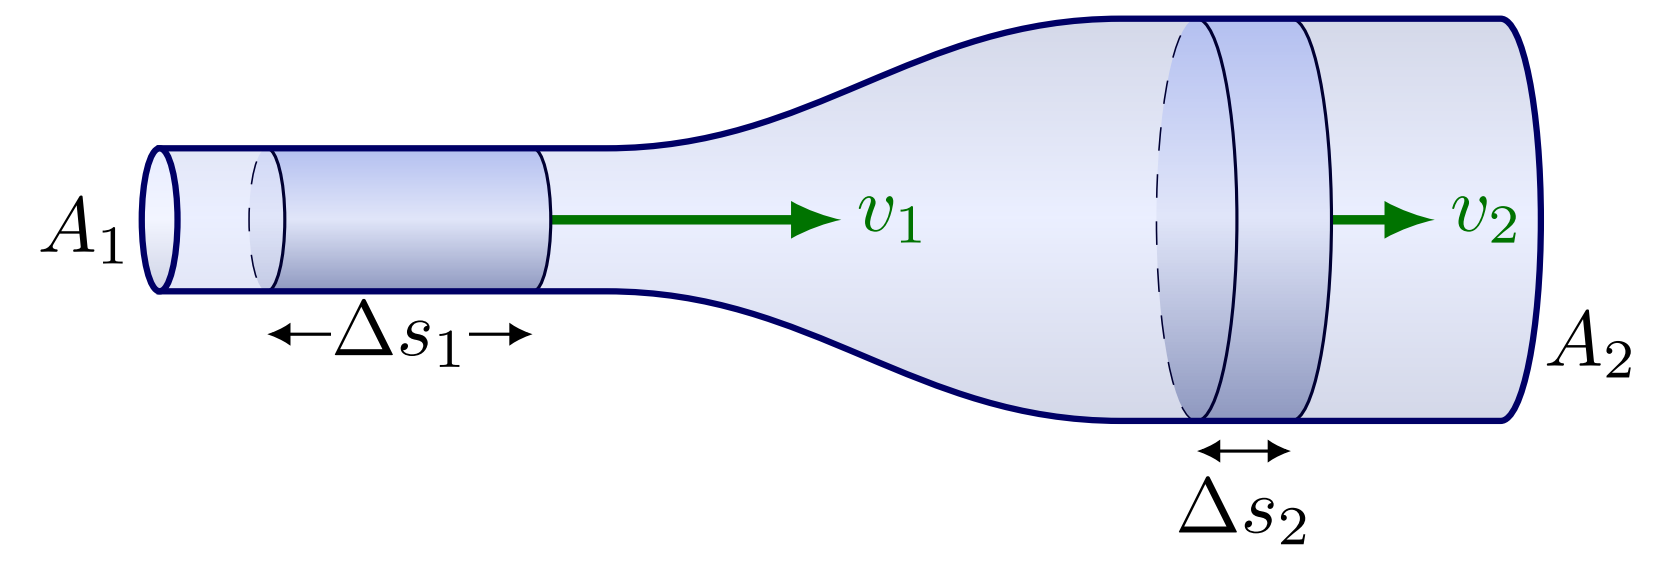
\includegraphics[width=0.9\columnwidth, align=c]{images/Kontinuitaet.png}
\end{center}

Die Kontinuitätsgleichung beschreibt die Erhaltung des Volumenstroms in einer strömenden Flüssigkeit:

$
\boxed{
    Q = A \cdot v 
} 
\quad
\boxed{
    Q_1 = Q_2 
} 
\quad
\boxed{
    A_1 \cdot v_1 = A_2 \cdot v_2
}
\quad
\boxed{
    Q = \dot{V} = \frac{\Delta V}{\Delta t} = \text{const} 
} 
$

\renewcommand{\arraystretch}{1.2} % Erhöht Zeilenhöhe für bessere Lesbarkeit
\begin{tabular}{@{} l p{6cm} l @{}}
    $[Q_x]$        & Durchflussrate                     \dotfill & $\frac{m^3}{s}$ \\
    $[A_x]$        & Querschnittsfläche                 \dotfill & $m^2$ \\
    $[v_x]$        & Fliessgeschwindigkeit              \dotfill & $\frac{m}{s}$ \\
    $[\dot{V}]$    & Volumenstrom (Volumen pro Zeit)    \dotfill & $\frac{m^3}{s}$ \\
    $[\Delta V]$   & Volumenänderung                    \dotfill & $m^3$ \\
    $[\Delta t]$   & Zeitänderung                       \dotfill & $s$ \\
\end{tabular}



\subsection{Bernoulli-Druck-Gleichung für Speicherwasserkraftwerke}

\begin{center}
    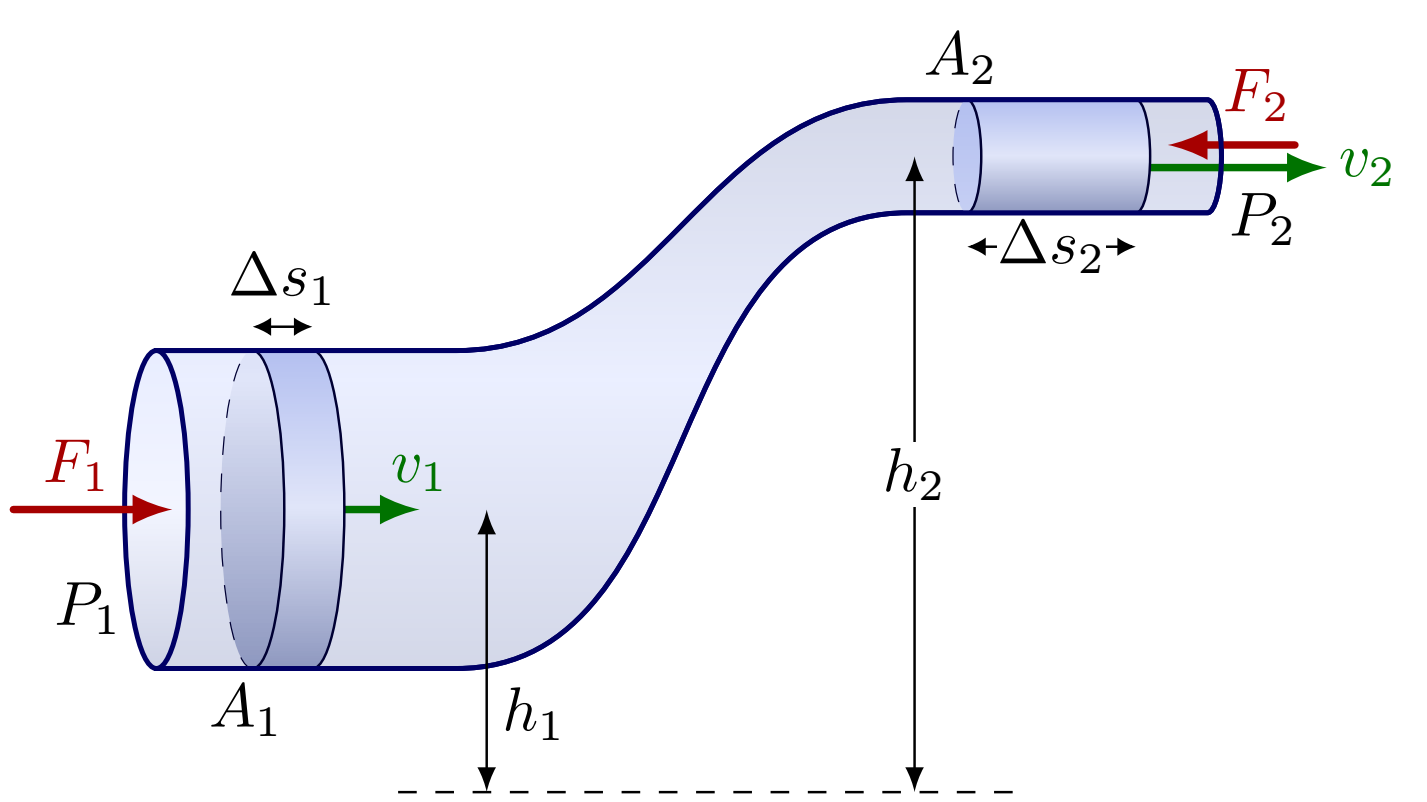
\includegraphics[width=0.9\columnwidth, align=c]{images/Bernoulli.png}
\end{center}

$\boxed{\frac{1}{2} \cdot \rho \cdot v^2 + \rho \cdot g \cdot z + p = \text{constant}}$

$
\boxed{
p_1 + \rho \cdot g \cdot h_1 + \frac{1}{2} \rho \cdot v_1^2 
= 
p_2 + \rho \cdot g \cdot h_2 + \frac{1}{2} \rho \cdot v_2^2
}
$

\renewcommand{\arraystretch}{1.2} % Erhöht Zeilenhöhe für bessere Lesbarkeit
\begin{tabular}{@{} l p {6cm} l @{}}
    $[\frac{1}{2} \rho v^2]$ & Kinetische Energie (je Kubikmeter) \dotfill & $\frac{J}{m^3}$ \\
    $[\rho g z]$             & Potentielle Energie                 \dotfill & $\frac{J}{m^3}$ \\
    $[p]$                    & Druckenergie                        \dotfill & $\frac{J}{m^3}$ \\
\end{tabular}


$
\underbrace{p}_{A} + \underbrace{\rho g z}_{B} + \underbrace{\frac{1}{2}\rho v^2}_{C} = \underbrace{\text{constant}}_{D}
$


\subsection{Bernoulli-Höhen-Gleichung für Speicherwasserkraftwerke}

$\boxed{H = z + \frac{p}{\rho \cdot g} + \frac{v^2}{2 \cdot g} + \sum H_v}$

\renewcommand{\arraystretch}{1.2} % Erhöht Zeilenhöhe für bessere Lesbarkeit
\begin{tabular}{@{} l p {4cm} l @{}}
    $[H]$                           & Bruttogefälle                              \dotfill & $m$ \\
    $[z]$                           & Höhenlage (potenzielle Energie)            \dotfill & $m$ \\
    $[p]$                           & Druck                                      \dotfill & $Pa = \frac{N}{m^2}$ \\
    $[\rho]$                        & Dichte des Wassers                         \dotfill & $\frac{kg}{m^3}$ \\
    $[g]$                           & Erdbeschleunigung                          \dotfill & $\frac{m}{s^2}$ \\
    $[v]$                           & Geschwindigkeit                            \dotfill & $\frac{m}{s}$ \\
    $\left[\frac{p}{\rho g}\right]$ & Druckhöhe                                  \dotfill & $m$ \\
    $\left[\frac{v^2}{2g}\right]$   & Geschwindigkeitshöhe                       \dotfill & $m$ \\
    $[\sum H_v]$                    & Hydraulische Energieverluste               \dotfill & $m$ \\
\end{tabular}


\subsection{Örtliche Energieverluste}

$\boxed{h_v = \zeta \cdot \frac{v^2}{2g}}$

\renewcommand{\arraystretch}{1.2} % Erhöht Zeilenhöhe für bessere Lesbarkeit
\begin{tabular}{@{} l p {4cm} l @{}}
    $[h_v]$     & Örtliche Energieverlusthöhe   \dotfill & $m$ \\
    $[\zeta]$   & Verlustbeiwert (dimensionslos) \dotfill & $-$ \\
    $[v]$       & Geschwindigkeit               \dotfill & $\frac{m}{s}$ \\
    $[g]$       & Erdbeschleunigung             \dotfill & $\frac{m}{s^2}$ \\
\end{tabular}


\subsection{Reibungsverluste}

$\boxed{H_{\text{vr}} = \frac{v^2 \cdot L}{K^2 \cdot R_h^{4/3}}}$

\renewcommand{\arraystretch}{1.2} % Erhöht Zeilenhöhe für bessere Lesbarkeit
\begin{tabular}{@{} l p {4cm} l @{}}
    $[H_{\text{vr}}]$  & Reibungsverlusthöhe      \dotfill & $m$ \\
    $[v]$              & Strömungsgeschwindigkeit \dotfill & $\frac{m}{s}$ \\
    $[L]$              & Länge der Strömungsstrecke \dotfill & $m$ \\
    $[K]$              & Rauhigkeitsbeiwert nach Strickler \dotfill & $m^{1/3}/s$ \\
    $[R_h]$            & Hydraulischer Radius     \dotfill & $m$ \\
\end{tabular}


\subsubsection{Tabelle Rauhigkeitsbeiwert K}
\begin{tabular}{|l|l|c|}
    \hline
    \textbf{Material} & \textbf{Zustand} & \textbf{K [m$^{1/3}$/s]} \\
    \hline
    Stahl & neu & 75 \\
    \hline
    Stahl & schlechter Zustand, verrostet, verkrustet & 60 \\
    \hline
    Beton & glatt & 85 \\
    \hline
    Beton & rauh & 60 \\
    \hline
    PE, PVC &  & 100 \\
    \hline
\end{tabular}

\columnbreak


\subsubsection{Hydraulischer Radius}

\begin{minipage}[c]{0.48\columnwidth}
    \myul{\textbf{Rechteckqueerschnitt}}\\
    \begin{center}
        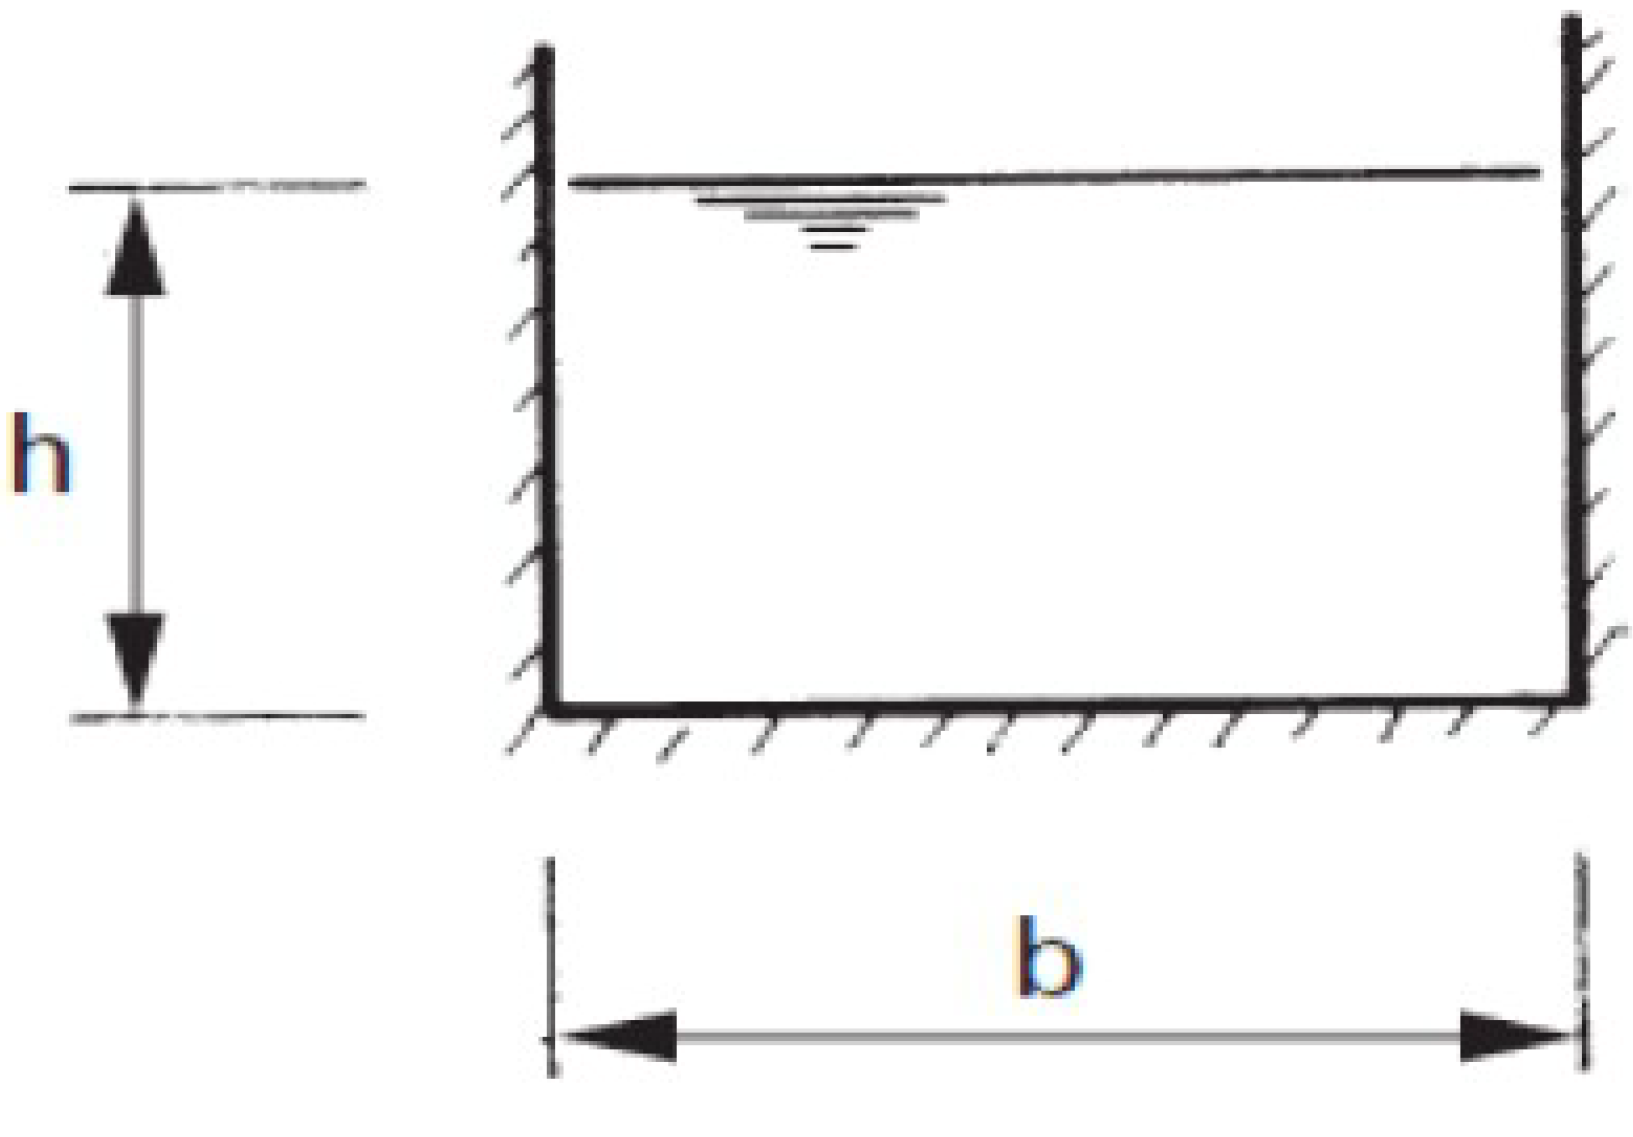
\includegraphics[width=0.9\textwidth, align=c]{images/Hydraulischer_Radius_Rechteck.png}
    \end{center}
\end{minipage}
\hfill
\vrule width 1pt % Vertikale Trennlinie mit 1pt Breite
\hfill
\begin{minipage}[c]{0.48\columnwidth}
    \myul{\textbf{Kreisqueerschnitt}}\\
    \begin{center}
        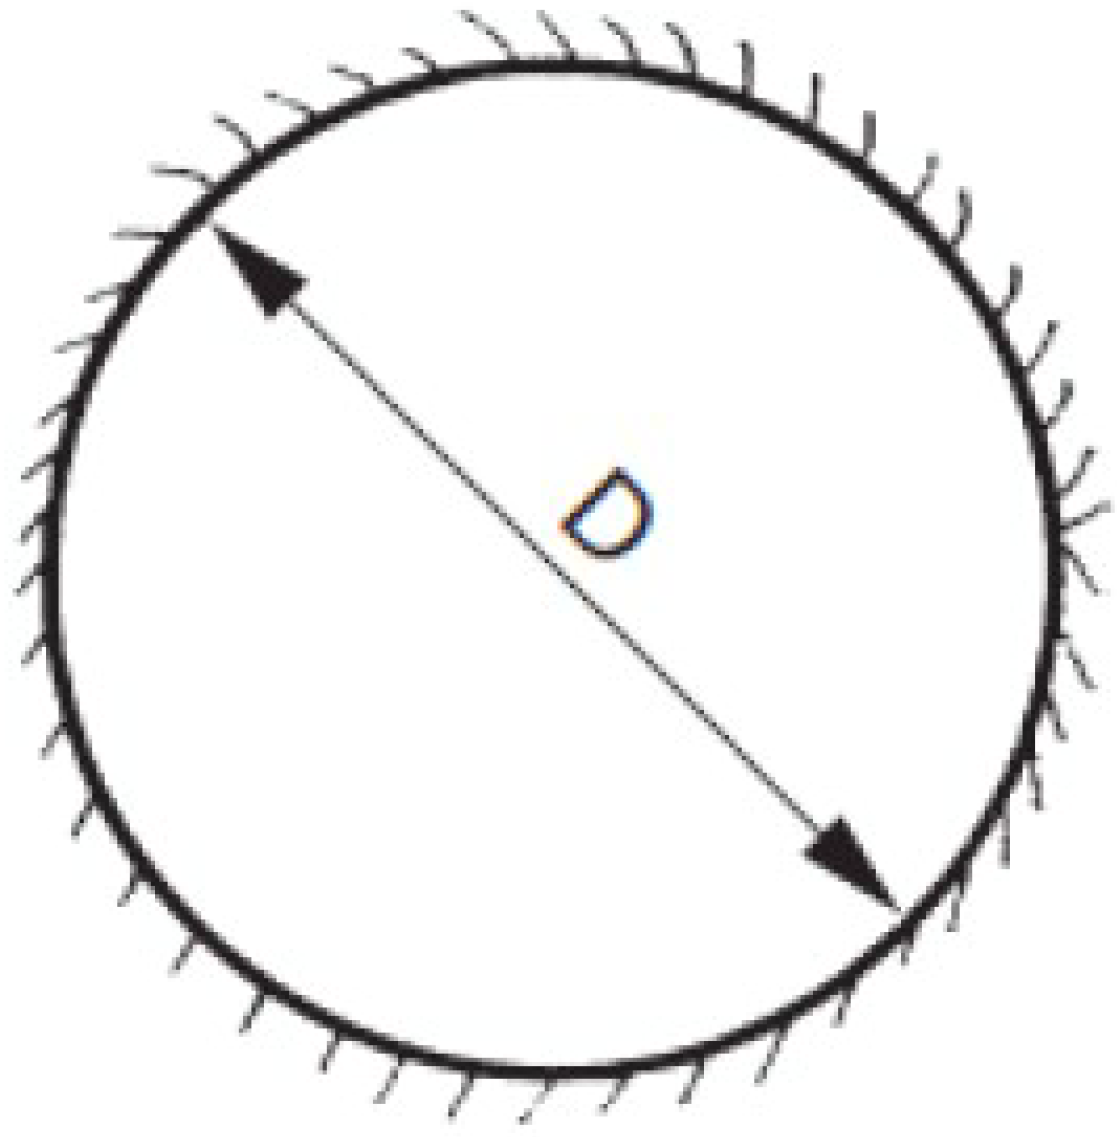
\includegraphics[width=0.65\textwidth, align=c]{images/Hydraulischer_Radius_Kreis.png}
    \end{center}
\end{minipage}

\vspace{0.25cm}

\begin{minipage}[c]{0.48\columnwidth}
    $\boxed{F = b \cdot h}$\\
    $\boxed{P = b + 2 \cdot h}$\\
    $\boxed{R_h = \frac{b \cdot h}{b + 2 \cdot h}}$ $\boxed{R_h = \frac{F}{P}}$
\end{minipage}
\hfill
\vrule width 1pt % Vertikale Trennlinie mit 1pt Breite
\hfill
\begin{minipage}[c]{0.48\columnwidth}
    $\boxed{F = \frac{D^2 \cdot \pi}{4}}$\\
    $\boxed{P = D \cdot \pi}$\\
    $\boxed{R_h = \frac{D}{4}}$ $\boxed{R_h = \frac{F}{P}}$
\end{minipage}

\renewcommand{\arraystretch}{1.2} % Erhöht Zeilenhöhe für bessere Lesbarkeit
\begin{tabular}{@{} l p {6cm} l @{}}
    $[F]$    & Abflussquerschnittsfläche         \dotfill & $m^2$ \\
    $[P]$    & Benetzter Umfang                  \dotfill & $m$ \\
    $[R_h]$  & Hydraulischer Radius              \dotfill & $m$ \\
\end{tabular}




\subsection{Verlusthöhe durch Reibung}

$\boxed{h_{\text{v,r}} = \lambda \cdot \frac{L}{d_{\text{hy}}} \cdot \frac{v^2}{2 \cdot g} }$
$\boxed{h_{\text{v,r}} = \lambda \cdot \frac{L}{d_i} \cdot \frac{8 \cdot Q^2}{g \cdot \pi^2 \cdot d_i^4}}$
$\boxed{h_{\text{v,r}} = \frac{8 \cdot \lambda \cdot L \cdot Q^2}{g \cdot \pi^2 \cdot d_i^5}}$

\renewcommand{\arraystretch}{1.2} % Erhöht Zeilenhöhe für bessere Lesbarkeit
\begin{tabular}{@{} l p {6cm} l @{}}
    $[h_{\text{v,r}}]$  & Verlusthöhe durch Reibung      \dotfill & $m$ \\
    $[L]$               & Länge                          \dotfill & $m$ \\
    $[v_m]$             & Mittlere Geschwindigkeit      \dotfill & $\frac{m}{s}$ \\
    $[Q]$               & Durchfluss                     \dotfill & $\frac{m^3}{s}$ \\
    $[d_i]$             & Innendurchmesser               \dotfill & $m$ \\
    $[d_{\text{hy}}]$   & Hydraulischer Durchmesser      \dotfill & $m$ \\
    $[l_u]$             & Benetzter Umfang               \dotfill & $m$ \\
    $[\lambda]$         & Verlustbeiwert                 \dotfill & $-$ \\
\end{tabular}

Zusammenhang des hydraulischen Durchmessers:

\[
d_{\text{hy}} = d_{\text{Kreisrohr}} = d_i = 4 R_{\text{hy}} = 4 \left(\frac{A}{l_u}\right)
\]



\subsection{Reynolds-Zahl $\text{Re}$}

Die Reynolds-Zahl $\text{Re}$ beschreibt das Verhältnis von Trägheitskräften zu Zähigkeitskräften in einer Strömung und wird wie folgt berechnet:


$\boxed{\text{Re} = \frac{v_m \cdot d_{\text{hy}}}{\nu}}$

\vspace{0.25cm}

Bemerkung: $d_{\text{hy}} = d_{\text{Kreisrohr}} = d_i$

\renewcommand{\arraystretch}{1.2} % Erhöht Zeilenhöhe für bessere Lesbarkeit
\begin{tabular}{@{} l p {6cm} l @{}}
    $[\text{Re}]$   & Reynolds-Zahl (dimensionslos)          \dotfill & $-$ \\
    $[v_m]$         & Mittlere Strömungsgeschwindigkeit       \dotfill & $\frac{m}{s}$ \\
    $[d_{\text{hy}}]$ & Hydraulischer Durchmesser             \dotfill & $m$ \\
    $[d_i]$         & Innendurchmesser (für Kreisrohr gleich $d_{\text{hy}}$) \dotfill & $m$ \\
    $[\nu]$         & Kinematische Viskosität                 \dotfill & $\frac{m^2}{s}$ \\
\end{tabular}



















































































